\section{Datensatz}
\label{Datensatz}

Die verwendeten Daten stammen aus dem \textit{KIT Energy Smart Home Lab (ESHL)}. Das ESHL ist ein $60 m^2$ Apartment mit intelligenten Haushaltsger"aten und soll einen zuk"unftigen Haushalt simulieren. Die Daten des ESHL wurden "uber fast 3 Jahre zwischen dem 22.08.2011 und dem 31.07.2014 aufgezeichnet, weisen aber einige L"ucken auf. F"ur die Messungen wurden mehrere Stromz"ahler verwendet, bei Gro{\ss}verbrauchern wie etwa dem Boiler wurden dabei alle drei Phasen gemessen, sie sind durch die Anschlussnummer des Stromz"ahlers in den Daten identifizierbar. Bei den restlichen Ger"aten wurde nur je eine Phase gemessen, das hei{\ss}t, dass  3 unterschiedliche Ger"ate an einem Stromz"ahler angeschlossen sind. Sie sind durch die Nummer des Stromz"alers in Kombination mit Nummer des verwendeten Anschlusses (Port) identifizierbar. Wie viele Phasen zur Messung eines Ger"ats verwendet wurden l"asst sich dem Kommunikationsgateway (Controller) entnehmen.
Tabelle~\ref{uuid} zeigt die beschriebene Zuordnung von Ger"aten zu Stromz"ahler und Anschluss.
\begin{table}[h]
\begin{tabular}{l|l|l|l|l|l}
UUID & Name & Klassifikation & Controller & Meter & Port \\
\hline
...-5602c0a80114 & DRYER & APPLIANCE & 1 & 3 & 0 \\
...-5604c0a80114 & WASHINGMACHINE & APPLIANCE & 1 & 7 & 2
\end{tabular}
\caption["Ubersicht Ger"atezuordnung]{Beispiele f"ur Ger"atezuordnung, die Waschmaschine ist an (Smart-)Meter 7 Port 2 angeschlossen.}
\label{uuid}
\end{table}



\subsection{Gemessene Daten}
\label{Gemessene Daten}

Die Daten des \textit{KIT Energy Smart Home Lab} besitzen folgendes Format (Tabelle~\ref{formateshl}). \\
\begin{table}[h]
\begin{tabular}{l|l|p{1cm}|p{1cm}|p{1cm}|p{1cm}|p{1cm}|p{1.2cm}|p{2cm}}
Unixtime & UUID & Con-troller & Meter & Port & Span-nung & Strom-st"arke & Wirk-leistung & Z"ahlerstand \\
\hline
1382291846 & ...-5604c0a80114 & 1 & 7 & 2 & 218.5 & 8.96 & 1956 & 145550  \\
1315269463 & ...-5602c0a80114 & 1 & 3 & 0 & 223.8 & 13.16 & 2950 & 38300 \\
1315269465 & ...-5602c0a80114 & 1 & 3 & 0 & 223.9 & 12.5 & 2796 & 38300
\end{tabular}
\caption[Format ESHL Daten]{Format ESHL Datensatz.}
\label{formateshl}
\end{table}

Controller, Meter und Port werden, wie oben beschrieben, verwendet, um einen Datenpunkt einen eindeutigen Ger"at zuzuordnen. Hier ist zu beachten, sich diese Werte immer nur gemeinsam verwendet werden d"urfen, nur so ist eine eindeutige Identifizierung eines Ger"ates m"oglich.
Die Spalte mit der UUID-Zuordnung wird ignoriert, denn sie enth"alt ebenfalls die Information um welches Ger"at es sich handelt und ist somit redundant zu Controller, Meter und Port. \\
Ein Datenpunkt enth"alt die gemessene Spannung, die Stromst"arke und die Wirkleistung. Es wird zus"atzlich die aggregierte Wirkleistung (Z"ahlerstand) gemessen, welche aber zun"achst ignoriert wird, da sie sich aus der Wirkleistung berechnen l"asst. \\
Eine Besonderheit stellt das Aufzeichnungsintervall dar. Die Stromz"ahler erzeugen jede Sekunde einen neuen Datenpunkt f"ur jeden Anschluss, dieser wird aber nur gespeichert, wenn sich die Wirkleistung im Vergleich zum letzten gespeicherten Punkt um 5 Watt Wirkleistung unterscheidet. So werden insbesondere lange \textit{Off} Phasen auf einen Datenpunkt komprimiert, es gehen aber auch kleinere Schwankungen in der Wirkleistung von sehr verbrauchsarmen Ger"aten verloren.


\subsection{Berechnete Daten}
\label{Berechnete Daten}

Die Messung von Spannung und Stromst"arke erlaubt es eine Vielzahl von Energiewerten zu berechnen, in diesem Abschnitt werden die Schein- und Blindleistung vorgestellt, das Kapitel zur Vorverarbeitung wird zus"atzlich eine Form der Normalisierung vorstellen. 
Die Scheinleistung $S$ ist das Produkt aus Spannung $U$ und Stromst"arke $I$ und ist die gesamte, aus dem Netz gezogene Leistung:\\ $S = U * I$\\[0.5cm]
Zur Berechnung der Blindleistung $Q$ werden Schein- und Wirkleistung $P$ genutzt, die Blindleistung ist dabei Leistung, die aus dem Netz gezogen wird ohne tats"achlich genutzt zu werden:\\ $Q = \sqrt{S^2 - P^2}$ \\


\subsection{Die Waschmaschine}
\label{Die Waschmaschine}

Die Waschmaschine ist ein besonders interessantes Ger"at f"ur die Klassifikation, denn sie hat nicht nur einen \textit{On-} und einen \textit{Off-Zustand}, sondern einen Motor, der mit verschiedenen Drehzahlen laufen kann, ein Heizelement und eine Pumpe. F"ur die Waschmaschine existieren au{\ss}erdem einige annotierte Waschg"ange (Tabelle \ref{profile01458}), die als Trainingsdaten verwendet werden k"onnen.\\
\begin{table}[h]
\begin{tabular}{l|p{3.5cm}|p{3.5cm}|l|l}
Profil & Startzeit \newline (Unix time stamp) & Endzeit \newline (Unix time stamp) & Dauer (Sekunden) & Datum \\
\hline
Profil 0 & 1382290611 & 1382296244 & 5633 & 20.10.2013 \\
Profil 1 & 1382363246 & 1382369468 & 6222 & 21.10.2013 \\
Profil 4 & 1382900551 & 1382905960 & 5409 & 27.10.2013 \\
Profil 5 & 1383173215 & 1383180425 & 7210 & 30.10.2013 \\
Profil 8 & 1384066710 & 1384072260 & 5550 & 10.11.2013
\end{tabular}
\caption["Ubersicht Trainingsdaten]{"Ubersicht "uber die annotierten Waschg"ange, die als Trainingsdaten verwendet werden.}
\label{profile01458}
\end{table}\\
Die Waschg"ange sind mit sechs verschiedenen Klassen Sigma 0 bis Sigma 5 annotiert, Sigma 0 ist der \textit{Off-Zustand}. Sigma 1 ist ein normaler Schleudervorgang, hier sind Phasen mit 200-350 Watt und dazwischen kurze Pausen mit ca. 4 Watt Verbrauch typisch.
Sigma 2 ist ein Heizvorgang, dieser kennzeichnet sich durch einen Verbrauch "uber 1700 Watt.
Sigma 3 und Sigma 4 sind Pumpvorg"ange und werden durch Verbrauchspitzen von wenigen Sekunden charakterisiert. Unterschieden werden sie anhand der H"ohe der Spitze, ein Vorgang Sigma 4 folgt immer auf einen Vorgang Sigma 3 mit einem Abstand von 50 bis 80 Sekunden.
Sigma 5 ist das Ausschleudern, es ist ebenfalls ein Schleudervorgang, der aber im Gegensatz zu Sigma 1 ohne Pausen ausgef"uhrt wird. \\

Grafik~\ref{typWasch} veranschaulicht die Wertebereiche und Lage der Klassen innerhalb eines Waschgangs. Die Klassen sind dabei wie in der Legende beschrieben farbig markiert, da die dunkelblau  gef"arbte Klasse 0 typischerweise einen Verbrauch von 0 Watt aufweist verl"auft der Graph zu diesen Zeitpunkten auf der x-Achse. Die rot gekennzeichneten Abschnitte der Heizvorg"ange sind in der ersten H"alfte des Waschgangs zu finden, hier wird das Wasser zun"achst aufgew"armt und muss dann mehrfach nachgeheizt werden um die Temperatur zu halten. Die hellblau und lila markierten Abschnitte der Pumpvorg"ange befinden sich in der 2. H"alfte des Waschgangs. Sie sind sehr kurz und folgen in regelm"a{\ss}igen Abst"anden aufeinander. Der Ausschleudervorgang von Klasse 5 ist nahe dem Ende des Waschgangs zu finden, er ist gelb gekennzeichnet.
\begin{figure}[ht]
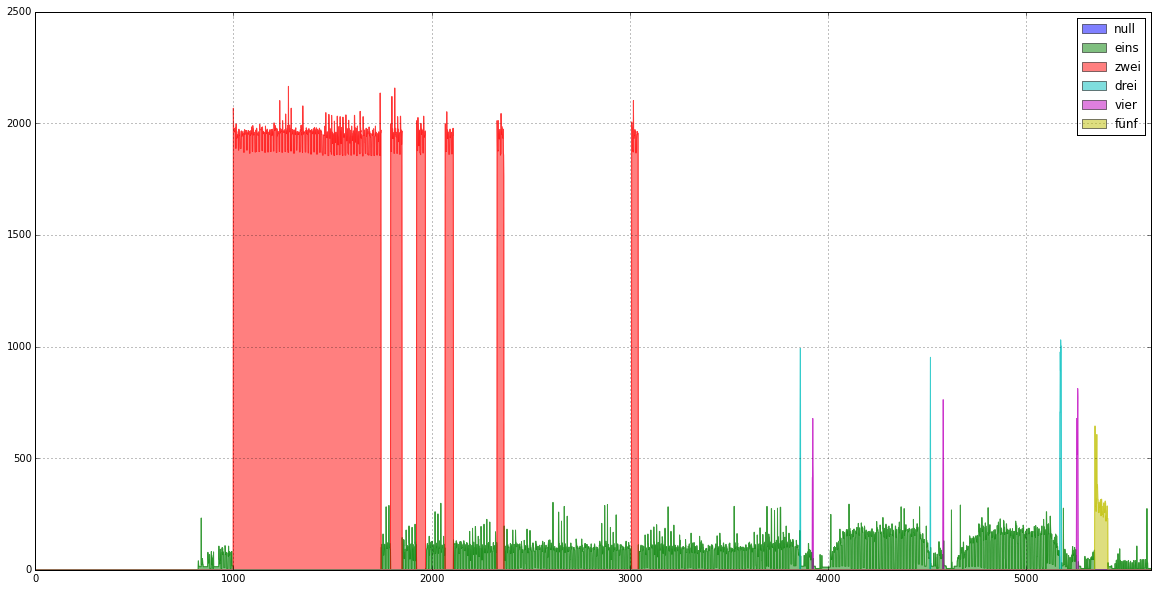
\includegraphics[height=0.7\textwidth , angle=90]{1_Grafiken/classes0.png}
	\caption[Typischer Waschgang, farbig annotiert]{Ein typischer Waschgang, je nach Klasse wird die Wirkleistung in unterschiedlichen Farben dargestellt}
\label{typWasch}
\end{figure}
